\chapter{Design og Implementering}

\section{Hardware}
I Goofy Candygun 3000 indgår forskellige hardwaredele, som skal udgøre det færdige system. Ud fra BDD'et ses det, at de to overordnede hardwaredele, der skal udvikles, er motorstyring til den vertikale og horisontale drejeretning, og en affyringsmekanisme. 

\subsection{Motorstyring af drejeretning}
For at kanonen kan sigte både vertikalt og horisontalt, skal den kunne køre i begge disse retninger. Det afhjælpes ved at bruge to DC-motorer - en til hver retning. Men for at disse så kan køre både forlæns og baglæns, skal der bruges en H-bro. For at sikre at motorerne ikke kan dreje 360 grader, er der udviklet en rotationsbegrænsning, som gør, at de kun kan dreje cirka 35 grader ud til hver side. 

\subsubsection{H-bro}
For at få mulighed for, at motoren både kan køre frem og bakke, skal der bruges en H-bro. I stedet for at bruge en færdig driver er der valgt at udvikle en selv. På figur \ref{fig:hbro} ses kredsløbsdiagrammet for H-broen. 

\begin{figure}[H]
	\begin{adjustwidth}{-3cm}{-\rightmargin}
		\centering
		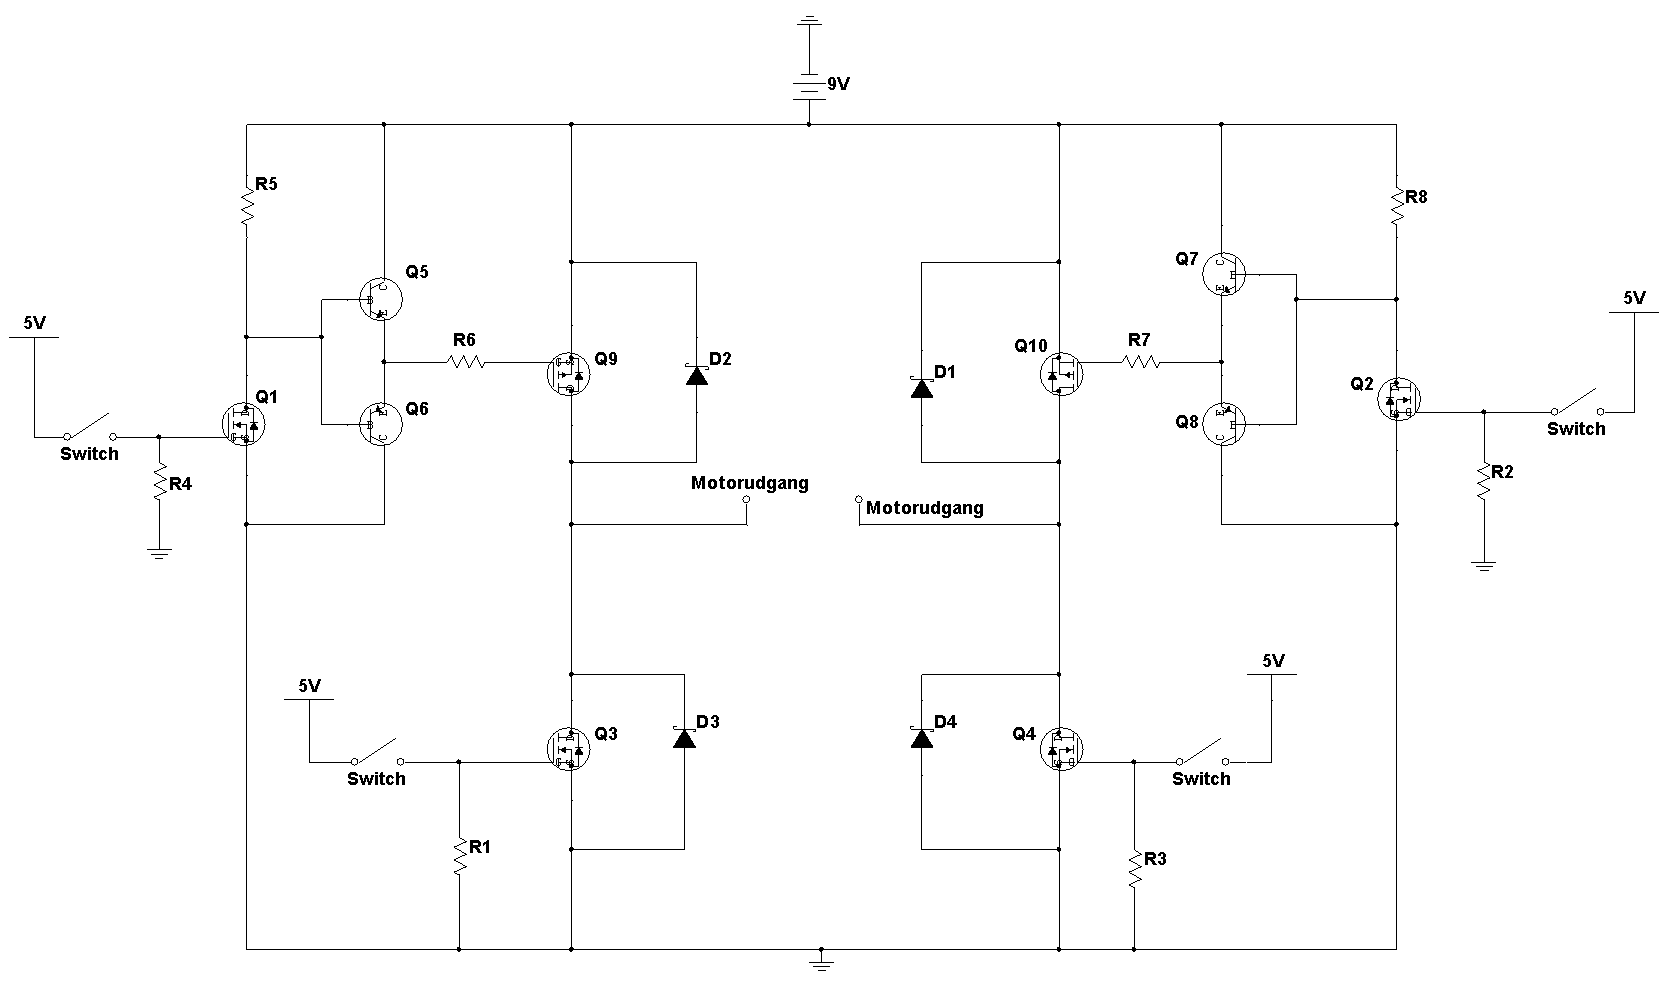
\includegraphics[width=0.9\paperwidth]{Afsnit/DesignOgImplementering/images/H-bro}
		\caption{Diagram af H-bro}
		\label{fig:hbro}
	\end{adjustwidth}
\end{figure}

\begin{table}[H]
	\centering
	\begin{tabular}{|l|l|l}
		\cline{1-2}
		\textbf{Betegnelse} & \textbf{Komponent}  	    &  \\ \cline{1-2}
		VCC        			& 5V                        &  \\ \cline{1-2}
		Q1   				& IRLZ44(mosfet N-Channel)  &  \\ \cline{1-2}
		Q2   				& IRLZ44(MOSFET N-kanal)	&  \\ \cline{1-2}
		Q3   				& IRLZ44(MOSFET N-kanal)	&  \\ \cline{1-2}
		Q4   				& IRLZ44(MOSFET N-kanal)	&  \\ \cline{1-2}
		Q5   				& BC547                     &  \\ \cline{1-2}
		Q6   				& BC557                     &  \\ \cline{1-2}
		Q7   				& BC547                     &  \\ \cline{1-2}
		Q8   				& BC557                     &  \\ \cline{1-2}
		Q9   				& IRF9Z34N(MOSFET P-kanal)	&  \\ \cline{1-2}
		Q10  				& IRF9Z34N(MOSFET P-kanal) 	&  \\ \cline{1-2}
	\end{tabular}
	\caption{Komponentbetegnelser på H-bro}
	\label{hbrotabel}
\end{table}

H-broen er bygget op af to identiske kredsløb - et til hver retning. Derfor beskrives kun den ene retning. Kredsløbet består grundlæggende af en N-MOSFET og en P-MOSFET. Når der sendes 5V ind på gate-benet til de to MOSFET's løber der en strøm gennem dem. Det betyder, at der bliver åbnet for, at motoren kan køre. I dette tilfælde skal motoren køre ved hjælp af et PWM-signal, så det betyder, at de to MOSFET's vil stå og åbne og lukke så lang tid, dette signal sendes ind. Det betyder også, at det er muligt, at styre motorens hastighed ved hjælp af PWM-signalets dutycycle. 

For at gøre det muligt, at motoren kan skifte retning hurtigt er der indsat to transistorer. Inden disse blev sat ind, blev P-MOSFET'en (Q9) opladet hurtigt men afladet meget langsomt. For at få den til at aflade hurtigt blev Q5 indsat. Det gjorde, at N-MOSFET'en (Q4) blev langsom til at oplade, så derfor blev Q6 sat ind. 

\subsubsection{Rotationsbegrænsning}
Motoren, som styrer platformen, skal kunne bevæge sig frit i intervallet, som er fastsat i kravspecifikationen \textbf{\#ref Reference til kravspecikation (ikke-funktionelle krav)}. For at begrænse denne bevægelse udenfor det fastsatte interval, anvendes der et potentiometer. Når motoren bevæger sig, ændres potentiometerets modstandsværdi, og dermed ændres spændingsniveauet. Altså kan motorens position bestemmes ved at se på outputspændingen fra potentiometret. Et alternativ til denne løsning er, at der anvendes en steppermotor, der kan styres i små steps, fremfor en DC-motor. Da der var et ønske om at arbejde med flere hardwareelementer end kun motoren, blev DC-motoren med rotationsbegrænsning valgt.

\begin{figure}[H]
	\centering
	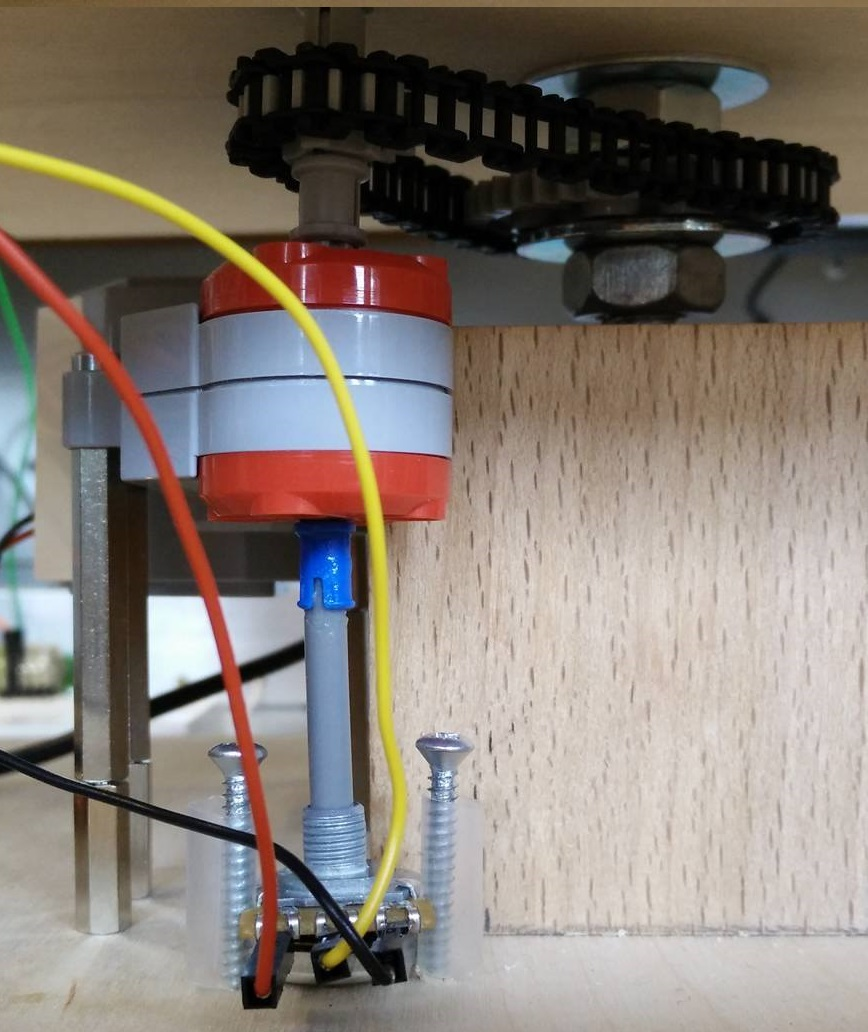
\includegraphics[scale=0.3]{Afsnit/DesignOgImplementering/images/potentiometerADC}
	\caption{Opstilling for rotationsbegrænsning}
	\label{fig:opstillingADC}
\end{figure}

\noindent På figur \ref{fig:opstillingADC} ses opstillingen for rotationsbegrænsningen. På figuren ses, at potententiometerets skaft er forbundet til motoren, som roterer når motoren bevæges. Potentiometeret bliver forsynet med 5V og stel fra PSoC1 via den røde og sorte ledning. Ouputspændingen fra potentiometeret er forbundet til PSoC1 via den gule ledning.  \newline

Potentiometeret har til formål at styre motoren i det definerede interval. Det valgte potentiometer er et lineært 47k\(\Omega\) potentiometer. Det vil sige, at for hver ændring, der sker i modstanden, vil der ske en proportional ændring i outputspændingen. Outputspændingen føres ind på et ben på PSoC'en, som er forbundet til en intern AD-converter, som er en Sequencing Successive Approximation ADC. Denne anvendes til at digitalisere det analoge signal fra potentiometeret.

En sequencing SAR ADC indeholder et sample-hold kredsløb og en comparator. Kredsløbet holder på et indgangssignal, indtil det næste signal registreres på kredsløbets indgang. Dermed har converteren tid til at bestemme resultatet af konverteringen. Comparatoren sammenligner inputsignalet med midscaleværdien. 

\begin{figure}[H]
	\centering
	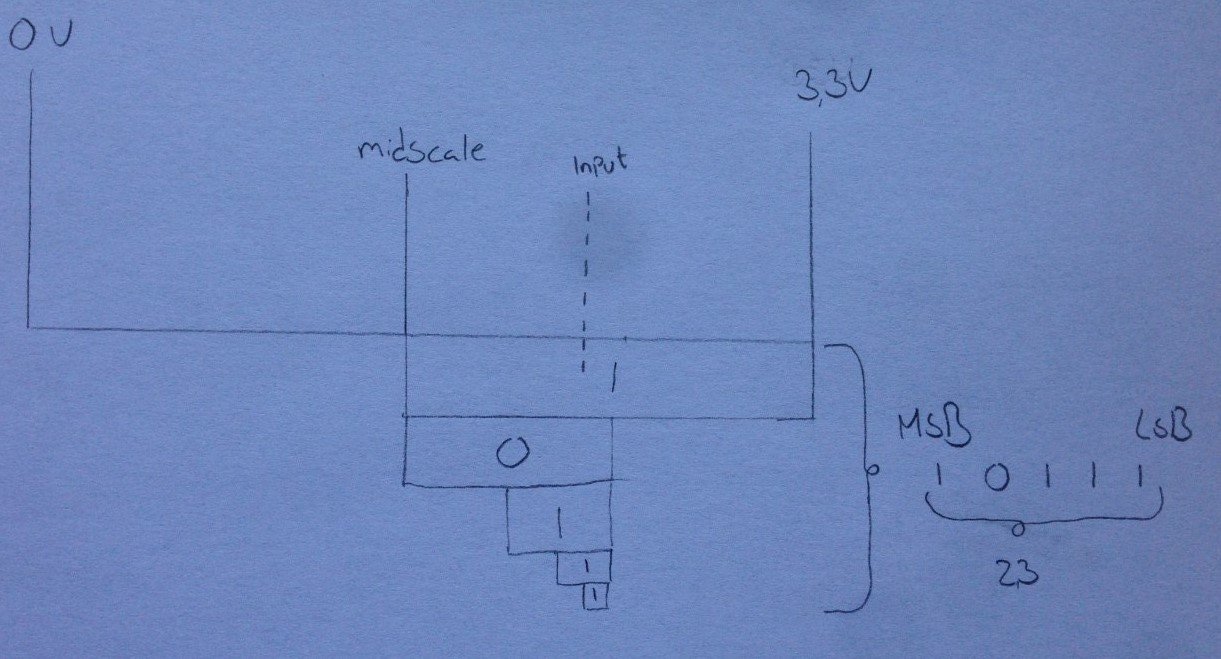
\includegraphics[width=\textwidth]{Afsnit/DesignOgImplementering/images/ADC}
	\caption{ADC opbygning}
	\label{fig:konvertering}
\end{figure}

På figur \ref{fig:konvertering} er ADC'en indstillet til midscale og bruger dette punkt til sammenligning med inputsignalet.  

ADC’en består af et sampleholdkredsløb. Det vil sige, at den ser på dataene indtil der er fundet en værdi, så der går noget tid imellem hver værdi, så der er sørget for, at der ikke bliver lavet oversamples og der ikke bliver lavet aliasering af det signal, som kommer ind i ADC’en. For at finde den værdi, som bliver sendt ind i ADC'en, bliver der lavet en skala, som bliver halveret alt efter, hvor værdien ligger på skalaen, som vist på figur \ref{fig:pot}

Der er blevet målt med en vinkelmåler for at overholde kravene i kravspecifikationen\textbf{\#ref Reference til kravspecikation (ikke funktionelle krav)}. Hvor der blev fundet frem til en minimum- og maksimumværdi, hvor motoren må køre imellem. \\
\\
Min=915 mV\\
\\
Max = 2000mV\\
\\
Disse værdier er aflæst fra PSoC’en. Da den har en referencespænding på 3.3V vil den have lavere værdier, end hvad der bliver sendt ud fra potentiometeret.
\begin{equation}
 \frac {5V} {3.3V}= 1.515
\end{equation}
Der er en forskel på cirka 1,515 mellem potentiometer og ADC. Så ADC er cirka 1,515 mindre end hvad potentiometer sender ud.
\\
For at forstå hvordan ADC’en og potentiometeret fungerer henvises til dokumentationen.


% % % % % % % % % Affyringsmekanisme % % % % % % % % % % % % % % % 
\subsection{Affyringsmekanisme}
Affyringsmekanismen består af en motor; et motorstyringskredsløb; et detektorkredsløb, der skal detektere, at motoren kun kører en enkelt omgang, når der skydes; og en kanon, som er bygget op af noget mekanik og LEGO. 

\subsubsection{Detektor}
Når kanonen affyres, styres det af motoren, og som mekanikken er opbygget, er der et propertionelt forhold mellem omdrejning på motoren og antal skud, der affyres. Derfor er det væsentligt at vide, hvornår motoren har roteret en runde, så den kan stoppes, inden der igen skydes. Til det formål anvendes detektoren. Billedet på figur \ref{fig:detektor} illustrerer hvordan detektoren anvendes.

\begin{figure}[H]
	\centering
	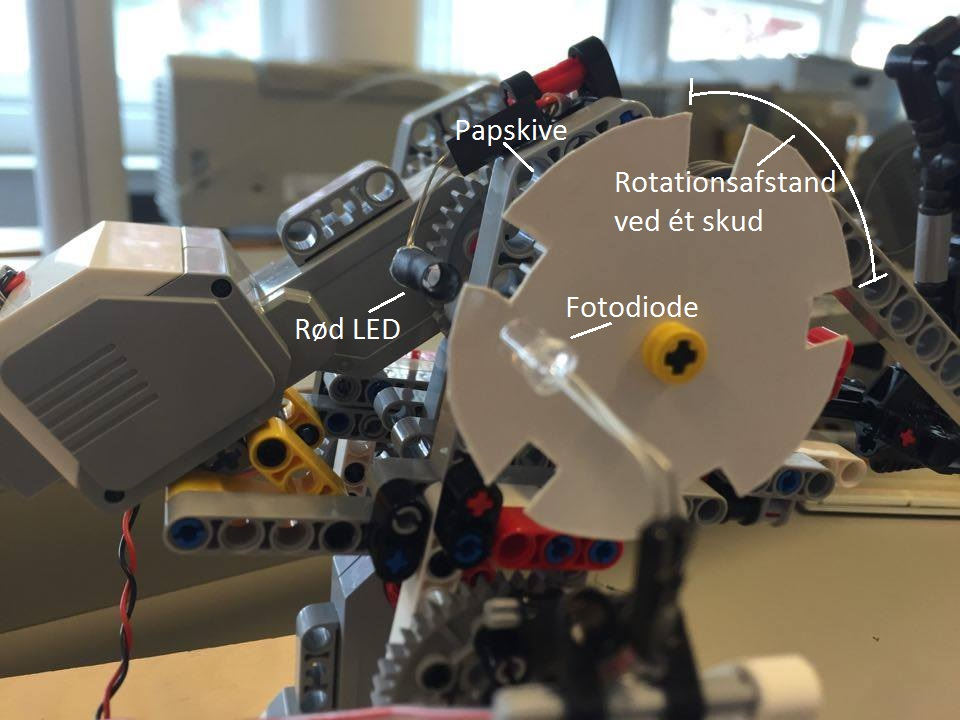
\includegraphics[width=\textwidth]{Afsnit/DesignOgImplementering/images/detektor}
	\caption{Detektorens placering på affyringsmekanismen}
	\label{fig:detektor}
\end{figure}

Den røde LED og fotodioden anbringes på affyringsmekanismen, som det ses på figur \ref{fig:detektor}. De vender ind mod hinanden, men er adskilt af papskiven. Papskiven er forbundet til motorens rotation, og hver gang et af papskivens hakker roterer forbi dioderne, kan de se hinanden. Fotodioden sender derefter et signal, som kan bruges til at stoppe motoren. Hvert hak passer med, at der er blevet affyret et skud.  

Detektoren skal kun sende et signal, når fotodioden ser lyset fra LED'en. Det er derfor vigtigt, at den ikke bliver forstyrret af dagslys og andre lyskilder. For at sikre dette, styres den røde LED af et PWM-signal, så LED'en blinker med en frekvens på 10 kHz. Detektoren opbygges tilsvarende af et båndpasfilter, med en centerfrekvens på 10 kHz, som sorterer andre frekvensområder og DC-signaler fra. 10 kHz er rigeligt højt, til at det for øjet ikke er synligt at LED'en blinker. Samtidig er det ikke for højt til, at en almindelig operationsforstærker kan håndtere det. På figur \ref*{fig:detektortand} ses et kredsløbsdiagram for detektoren og LED'en.

\begin{figure}[H]
	\centering
	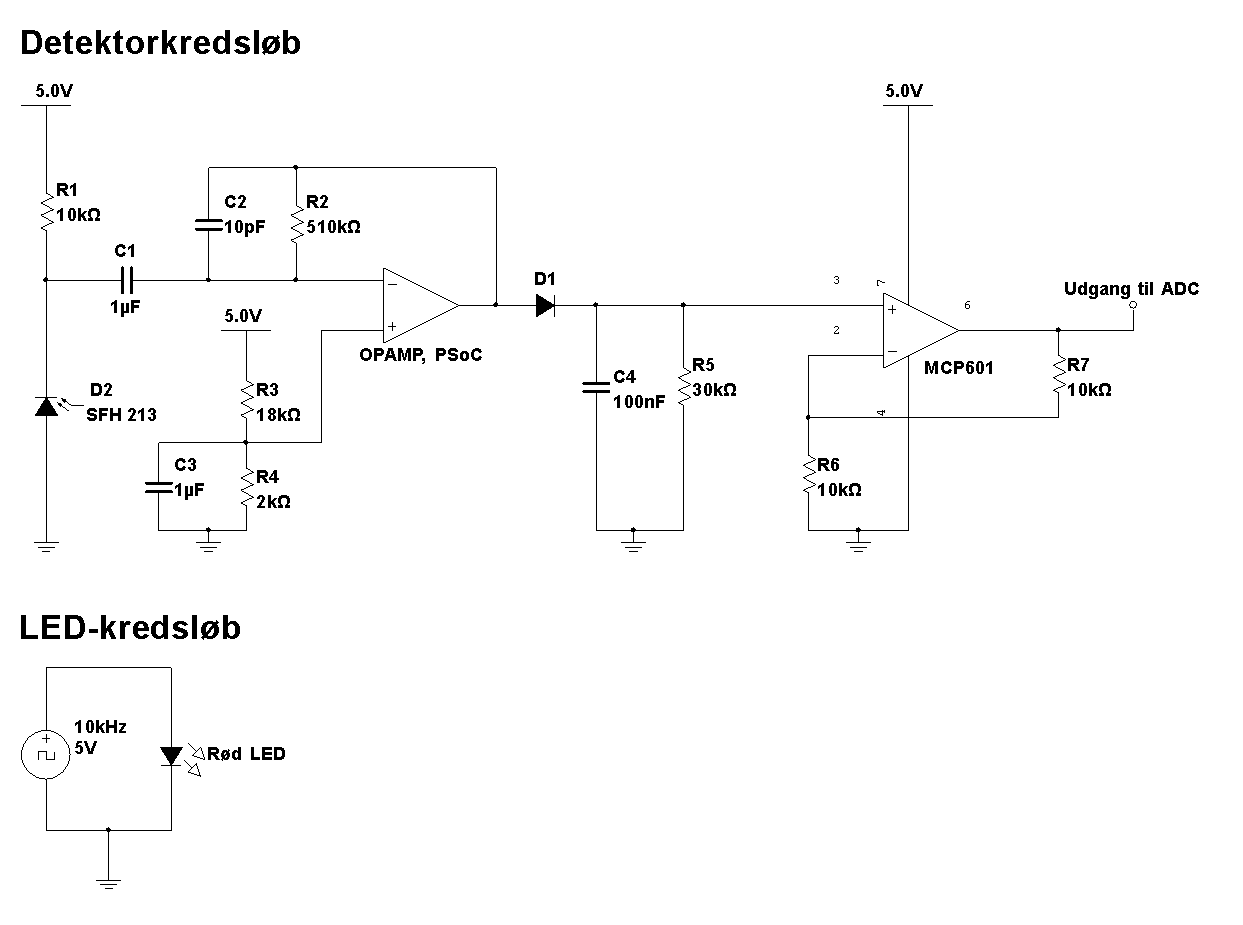
\includegraphics[width=\textwidth]{Afsnit/DesignOgImplementering/images/detektor_tandhjul}
	\caption{Kredsløbsdiagram for detektoren}
	\label{fig:detektortand}
\end{figure}

Båndpasfiltret er opbygget af et højpasfilter, et lavpasfilter og en operationsforstærker. Da PSoC'en har en indbygget operationsforstærker, anvendes denne. Software design og implementering af den ses under PSoC Software!!!! Af hensyn til operationsforstærkeren, er der valgt en referencespænding på 0,5 V på den positive indgang. Det er opnået ved en spændingsdeler, for hvilken beregningen kan ses i dokumentationen !!!!. Der er negativ feedback på operationsforstærkeren, hvilket sikrer, at der opretholdes samme spænding, 0,5 V, på begge indgange i operationsforstærkeren. Når fotodioden kan se den røde LED, genererer den en strøm, som bliver omsat til en spænding i kredsløbet. Operationsforstærkeren vil opretholde 0,5 V på den negative indgang. Den vil derfor regulere udgangen for at ophæve de ændringer, som fotodioden skaber på den negative indgang. Udgangssignalet vil dermed afspejle det PWM-signal, som den røde LED sender.  

Når fotodioden kan se lyset fra den røde LED er signalet, som kommer fra udgangen af operationsforstærkeren, et firkantsignal med en frekvens på 10 kHz,. Når fotodioden ikke kan se det røde lys, er spændingen på udgangen 0,5 V. Det ønskes omdannet til et signal, der går højt, når PWM-signalet starter, og går lavt, når PWM-signalet er væk igen. For at opnå dette, blev der lavet en envelopedetector, som er opbygget af en diode, en modstand og en kondensator. Dioden sikrer, at skulle der komme negative spændinger, så vil de blive frasorteret. Kondensatoren er dimentioneret efter, at den bliver opladet på de første udsving fra firkantsignalet. Modstanden er dimentioneret, så spændingen ikke aflades mellem svingningerne på 10 kHz signalet. En simulering af dette kan ses i dokumentationen !!!! 

Outputtet, fra envelopedetektoren var dog noget lavt. Det lå mellem 1,5V og 2V. Derfor blev der indsat en ikke-inverterende forstærker for at fordoble signalet. Forstærkeren består af en opamp og to modstande. Derfor blev der opstillet følgende ligning \ref{reference til Tores bog}: 

\begin{equation} 
	U_{O}=(1+\frac{R_{2}}{R_{1}})*U_{P}
\end{equation}

Det vil altså sige, at hvis de to modstande, der sættes ind er ens, vil indgangssignalet blive fordoblet. Hvis der eksempelvis sendes 2V ind vil der være 4V på udgangen: 

\begin{equation}
	U_{O}=(1+\frac{10k\Omega}{10k\Omega})*2V
\end{equation}

Herefter var det muligt at aflæse et tydeligt firkantsignal med en peak-to-peak-værdi på 3,5V. 

Den røde LED er koblet direkte til et 0-5 V, 10 kHz PWM signal fra PSoC'en. Den kan godt klare sig uden en formodstand. 

\subsubsection{Motorstyring}
Til at styre affyringsmekanismens motor er der bygget et kredsløb med en MOSFET som primære komponent. MOSFET'en skal sørge for, at motoren kun kører, når der bliver sendt PWM-signal ind i den. Kredsløbsdiagrammet kan ses på figur \ref{fig:affyringsmotor}. 

\begin{figure}[H]
	\centering
	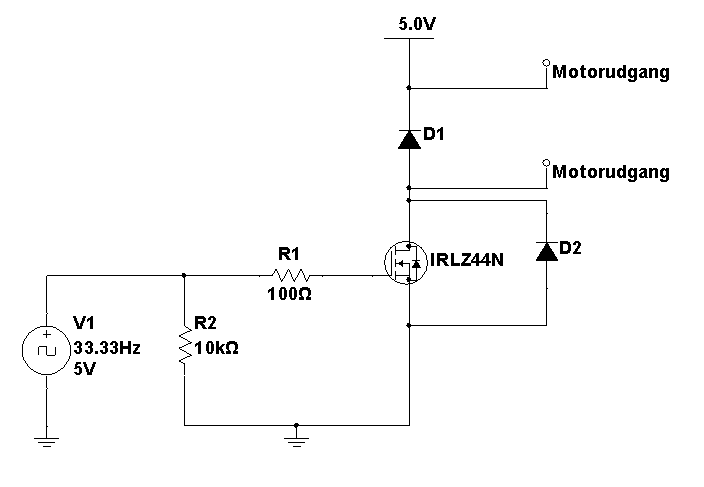
\includegraphics[width=0.7\textwidth]{Afsnit/DesignOgImplementering/images/motor_affyring}
	\caption{Diagram over motorstyring til motor på affyringsmekanisme}
	\label{fig:affyringsmotor}
\end{figure}

Dioden D1 er sat ind for at sikre motoren mod store spændingsspikes, der kan forekomme, når MOSFET'en bliver afbrudt. Dioden D2, der sidder fra source til drain, sikrer, at spikes genereret af motoren, når den slukkes, ikke brænder MOSFET'en af. 

\subsubsection{Kanon og platform}
Selve kanonen og platformen den står på er bygget op af to træplader og LEGO. Den ene træplade kan dreje fra side til side, således at det er muligt at sigte i den horisontale retning. Opbygningen ses på figur \ref{fig:Horisontalmekanik}. Træpladen placeres på den øverste metalskive omkring skruen, så den drejer med rundt, når motoren roterer. Rotationen er opnået ved, at skruen kan dreje frit, men stadig er holdt lodret. Det store tandhjul er boret ud i midten, og der er indsat en møtrik, så den kan skrues på skruen. Forholdet mellem det store og det lille tandhjul gør at rotationshastigheden bliver gearet ned. Endeligt er motoren skruet fast til den nederste træplade, men i en højde, der gør at den kan drive det lille tandhjul, som er forbundet med gearkæden til det store tandhjul. 

\begin{figure}[H]
	\centering
	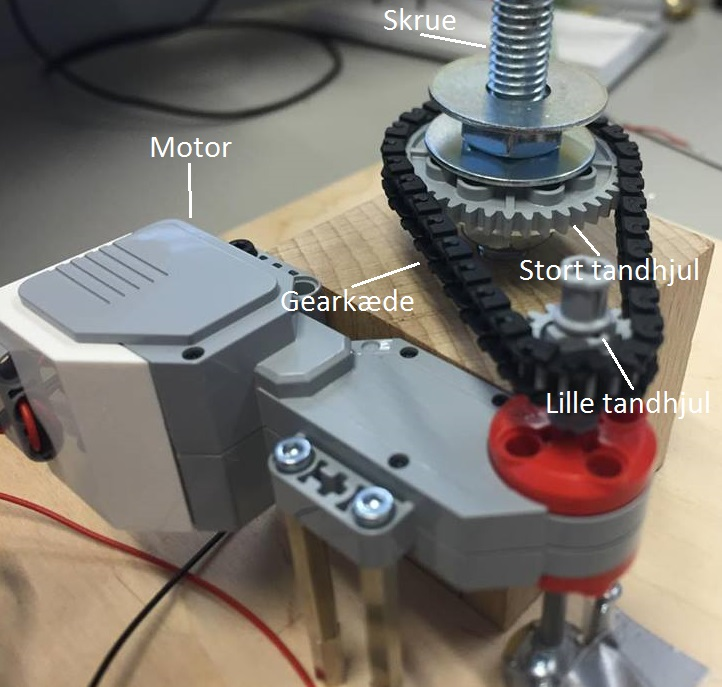
\includegraphics[width=1\textwidth]{Afsnit/DesignOgImplementering/images/horisontalMekanik}
	\caption{Horisontal mekanik}
	\label{fig:Horisontalmekanik}
\end{figure}

Mekanikken for den vertikale retning er bygget af LEGO. Et billede af opbygningen ses på figur \ref{fig:kanon}. Styringen af den vertikale bevægelse bliver håndteret af den vertikale motor, som ses på figur \ref{fig:kanon}. Motoren er forbundet til tandhjulene til vertikal styring. Der er ét tandhjul på hver side af motoren. De er begge bygget sammen med resten af kanonen. Når motoren drejer, bliver tandhjulene og hele kanonen vippet fremover eller bagover. 

Ligesom den vertikale styring er selve kanonen også bygget i LEGO. Den har et magasin, som det fremgår af figur \ref{fig:kanon}. Der kan kommes slik i magasinet, som så bliver affyret. Affyringen styres af den anden motor på figur \ref{fig:kanon}. Når affyringsmotoren drejer bliver to større tandhjul roteret. De to tandhjul er desuden forbundet til to små tandhjul, som er 5 gange så små. Med denne gearing roterer de små tandhjul 5 gange så hurtigt. De små tandhjul er forbundet til to mellem størrelse tandhjul, som drejer med dem rundt. Tandhjulene i mellemstørrelse styrer affyringen ved at omdanne den roterende bevægelse til en vandret bevægelse frem og tilbage, som affyrer kanonen.

\begin{figure}[H]
	\centering
	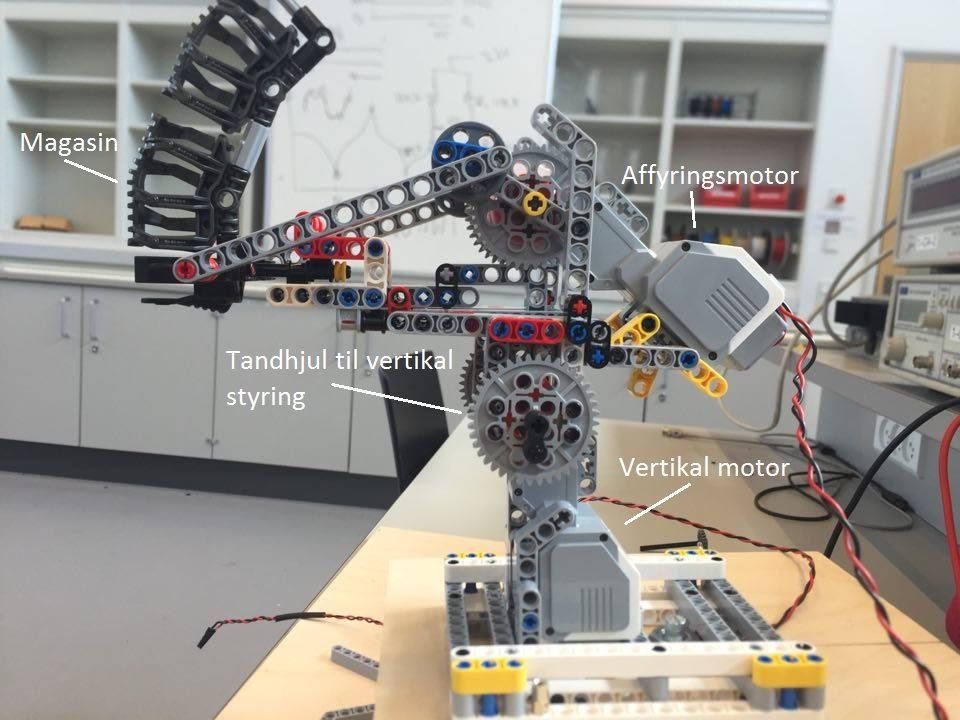
\includegraphics[width=1\textwidth]{Afsnit/DesignOgImplementering/images/kanon}
	\caption{Kanon i LEGO}
	\label{fig:kanon}
\end{figure}
 

\section{Software}

\subsection{SPI - Devkit8000}
Candydriveren sørger for SPI-kommunikationen fra Devkit8000 til PSoC0. Driveren er skrevet i c, hvilket er typisk for drivere til linuxplatforme.\\
SPI-kommunikationen er implementeret med SPI bus nummer 1, SPI chip-select 0 og en hastighed på 1 MHz (et godt stykke under max på 20 MHz for en sikkerhedsskyld). Desuden starter clocken højt og data ændres på falling edge og aflæses på rising edge. Dermed bliver SPI Clock Mode 3. Derudover sendes der 8 bit pr transmission, hvilket passer med SPI-protokollen for projektet.\\
For at kunne anvende driveren, når SPI er tilsluttet, er der oprettet et hotplugmodul, som fortæller kernen, at der er et SPI device, som matcher driveren. Det kan SPI-forbindelsen ikke selv gøre, som usb fx kan. Selve driveren er i candygun.c opbygget som en char driver. For at holde forskellige funktionaliteter adskilt er alle funktioner, der har med SPI at gøre, implementeret i filen candygun-spi-c. Så når der fx skal requestes en SPI ressource i init-funktionen i candygun.c, så anvender driveren en funktion fra candygun-spi.c til det. I probe-funktionen sættes bits\textunderscore per\textunderscore word til 8, da vi sender otte bit som nævnt tidligere. I exit-funktionen anvender candygun.c igen en funktion fra candygun-spi.c - denne gang til at frigive SPI ressourcen. I write-metoden gives der data med fra brugeren. I dette tilfælde udgøres brugeren af Interface driveren og dataet er en 8 bit kommando fra SPI-protokollen. Dog er dataet fra brugeren i første omgang læst ind som en charstreng. I write-metoden bliver det så lavet om til en int.  For at overføre dataet på en sikker måde anvendes funktionen copy\textunderscore from\textunderscore user() til at overføre data fra brugeren. Write-funktionen fra candygun.c anvender derefter en write-funktion fra candygun-spi.c, hvor den sender brugerinputtet med. I den spi-relaterede write-funktion bliver bruger inputtet lagt i transfer bufferen og der NULL bliver lagt i receive bufferen, og med spi\textunderscore sync-funktionen bliver det sendt.\\ 
Ofte ville der en spi read-funktion først indeholde en write-del, som fortalte SPI-slaven, hvad der skulle læses over i bufferen. Det ville typisk efterfølges af et delay og så en read-del. Men i dette projekt skal der ofte afventes et brugerinput, som ikke kan styres af et fast delay, og der skal generelt sendes en aktiv kommando før der læses. Derfor er det besluttet at read-funktionen kun indeholder en read-del i transmissionen. Dermed skal write-funktionen altid aktivt anvendes inden der læses, da PSoC0 ellers ikke ved, hvad der skal gøres/lægges i bufferen.\\
Når funktionen har modtaget resultatet fra transmissionen returneres det til brugeren med funktionen copy\textunderscore to\textunderscore user(), som igen sørger for at overførslen af data foregår på en sikker måde.   


\subsection{Interface Driver}
Interface driveren fungerer som bindeled mellem brugergrænsefladen og candydriveren på Devkit8000. Den indeholder tre funktioner. Funktionerne anvendes i use case 2 til at teste kommunikationsforbindelserne i resten af systemet. Interface driveren er designet og implementeret i C++ og gør brug af klasserelationen arv. Et klassediagram for interface driveren se på figur  \ref{fig:idriveruc2}.\\

\begin{figure}[H]
	\centering
	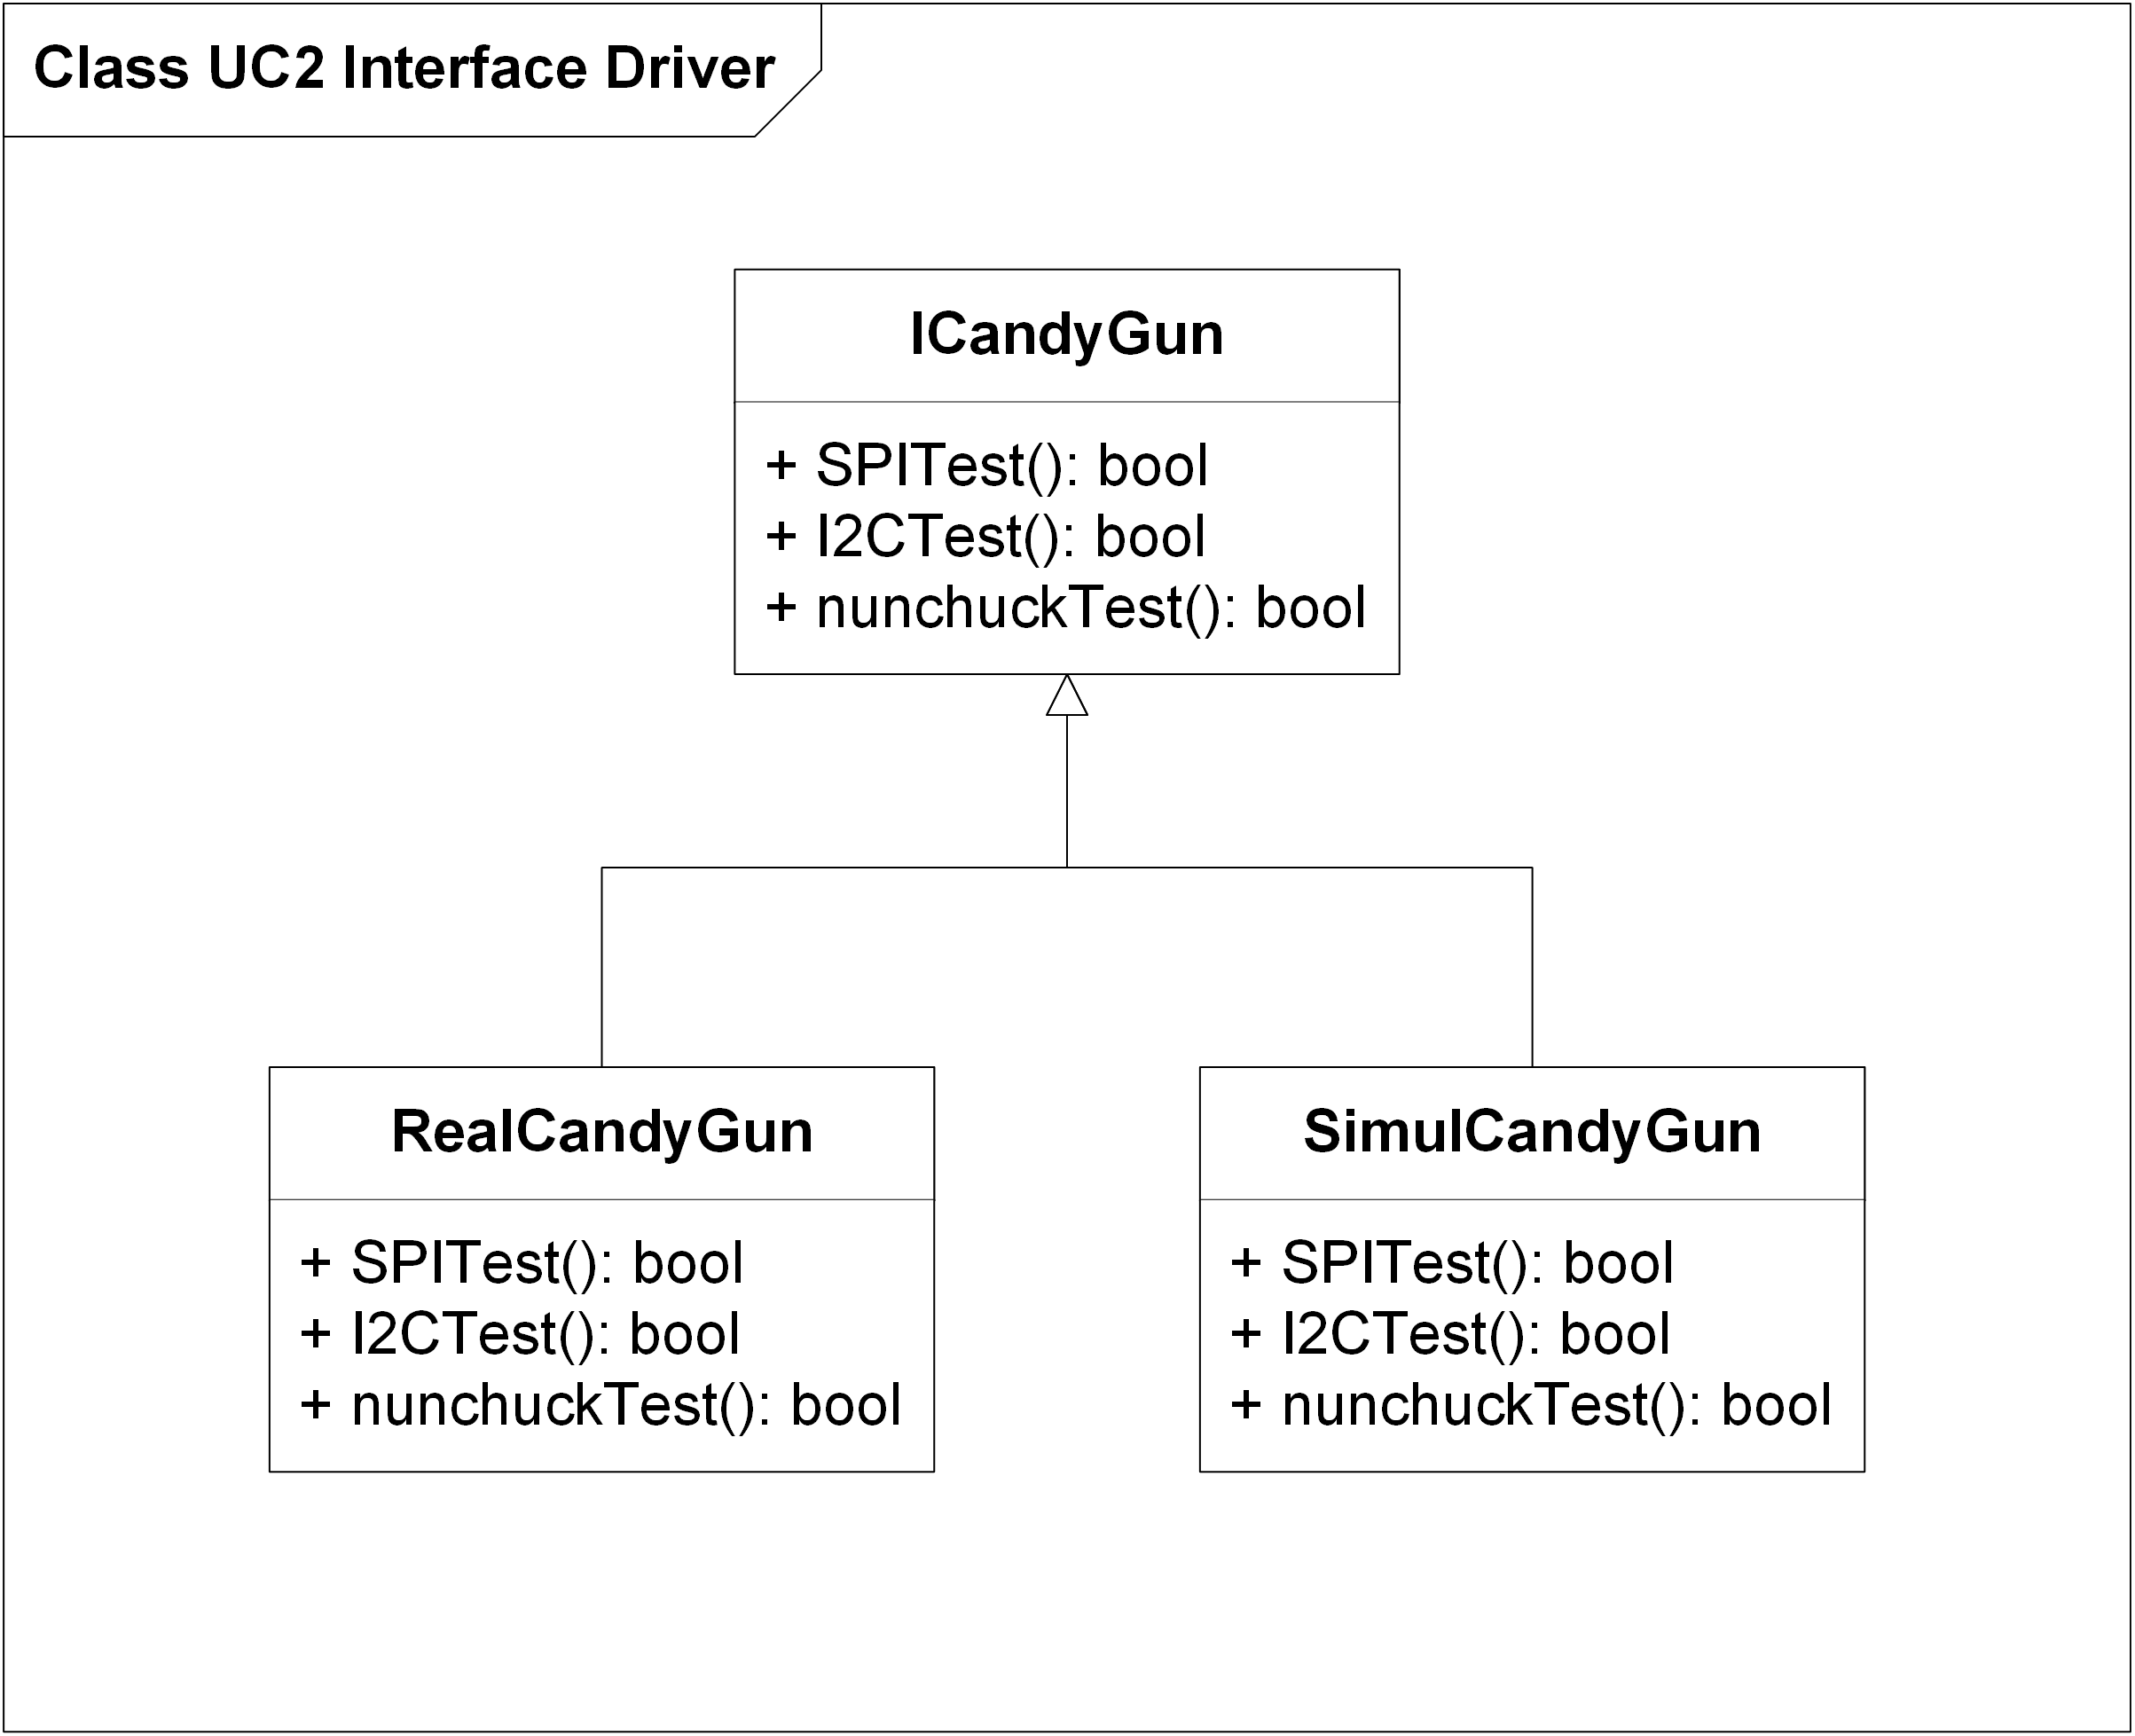
\includegraphics[width=\textwidth]{Afsnit/DesignOgImplementering/images/IdriverKlasseDiagram}
	\caption{Interface driver for UC2}
	\label{fig:idriveruc2}
\end{figure}

Basisklassen er ICandyGun. Det er en abstrakt klasse, da den udelukkende indeholder virtuelle metoder. Derudover er der to afledte klasser; SimulCandyGun og RealCandyGun. SimulCandyGun implementerer metoderne til at simulere respons fra Candydriveren. Dermed kan brugergrænsefladen testes uafhængigt af de resterende dele af systemet. Simuleringen er implementeret med \textit{srand()}-funktionen fra \textit{cstdlib}-biblioteket, som returnerer et tilfældigt tal, som her bliver mellem 0 og 1. I RealCandyGun-klassen er metoderne implementeret efter den reelle SPI-protokol og med de nødvendige funktioner til at skrive til et kernemodul. Fx open(), close(), read () og write(). Da interface driveren er implementeret med arv, skal der ikke foretages betydelige ændringer i brugergrænsefladen, når der skiftes mellem simuleringsklassen og den rigtige version. Dermed opnås lav kobling. \\
De tre funktioner som Interface driveren indeholder i forbindelse med use case 2 (test use casen) er: SPITest(), I2CTest(), NunchuckTest(). Hver af de tre funktioner anvendes til at starte en test af de forskellige kommunikationsforbindelser: SPI, I2C og brugerinputet fra nunchucken. Alle funktionerne returnerer en bool, som enten er true eller false, alt efter om testen var succesful eller ej. Når der skal startes en test, åbner den pågældende funktion filen \textit{dev/candygun} og skriver SPI-kommandoen for \textit{start test} til filen. Derefter venter funktionen ét sekund og læser så svaret fra filen. Da der i nunchucktesten ventes på et brugerinput, og brugeren skal have lidt tid til at trykke på nunchuck-knappen, er der oprettet en while-løkke, som tjekker flere gange om testen returnerer true. Hvis testen ikke returnerer true ved første check, venter funktionen atter et sekund og tjekker igen. Det gør den op til 15 gange og melder derefter om fejl, hvis ikke den returnerer true inden.\\
Brugergrænsefladen anvender interface driveren ved at inkludere headerfilerne og oprette en ICandyGun pointer, der peger på en instans af én af de to afledte klasser. Ved at pakke kommunikationen  til kernemodulet for candydriveren væk i funktioner kan brugergrænsefladen anvende funktionerne uden at kende til SPI-protokollen. Det sikrer igen lav kobling, og i tilfælde hvor det kunne ønskes, at SPI-kommunikationen kan erstattes af en anden kommunikationsform, kan det gøres uden, at der skal foretages ændringer i brugergrænsefladen.\\
 
\subsection{Brugergrænseflade}
Selve Usecase 2 styres via brugergrænsfladen fra Devkit8000.
Dette afsnit beskriver brugergrænsefladens design.

\begin{figure}[H]
	\centering
	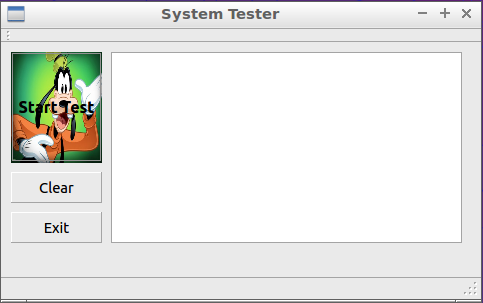
\includegraphics[width=\textwidth]{Afsnit/DesignOgImplementering/images/GUIPic}
	\caption{Brugergrænseflade for usecase 2}
	\label{fig:GUIPic}
\end{figure}

Brugergrænsefladen er lavet med det indbyggede design framework i QT Creator 5.
QT frameworket opretter "hovedvinduet" i brugergrænsefladen som en klasse. Knapperne tilføjes som private slots i klassen
hvilket gør dem i stand til interagere i brugergrænsefladen. Når en knap er assignet til et slot i klassen, og der trykkes på den pågældende knap, bliver det assignede signal broadcastet
og slot-funktionen bliver kørt. Alle tre knapper i brugergrænsefladen er assignet signal-typen "clicked()".

\begin{figure}[H]
	\centering
	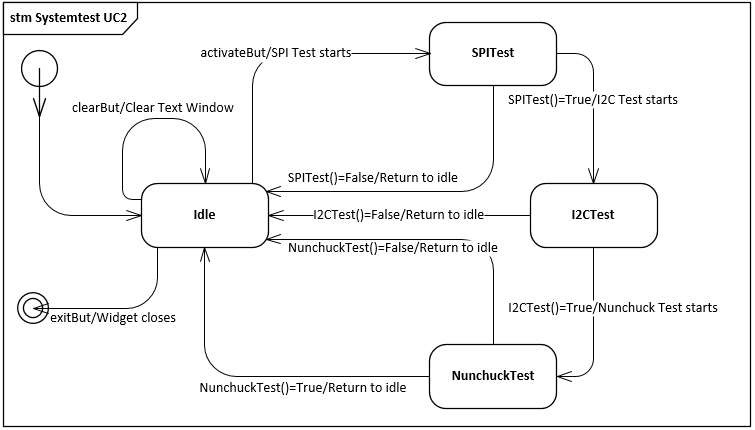
\includegraphics[width=1.2\textwidth]{Afsnit/DesignOgImplementering/images/StateMachineUC2}
	\caption{State machine for brugergrænsefladen for usecase 2}
	\label{fig:StateMachineUC2}
\end{figure}

Brugergrænsefladen for UC2 er en simpel test-konsol. Den består af 3 knapper og et tekstvindue. Brugergrænsefladen interfacer med SPI-protokollen, gennem vores interface driver. Den første knap, Start test, initierer UC2. Efterhånden som testen løbes igennem kaldes test funktionerne, og ved hjælp af if-conditions, bliver der tjekket på retur-værdierne fra interface-funktionerne. Hvis retur-værdien er true, skrives der en "--test successful" besked i tekstvinduet. og widgeten kører videre. Hvis retur-værdien er false, skrives der en "--test unsuccessful" i tekstvinduet og widgeten returnerer til idle tilstand. Når alle test er successful, skrives "System test successful, system is ready for use" til tekstvinduet, og widgeten returnerer til idle tilstand. Den anden knap, Clear, clearer tekstvinduet til blank tilstand. Den tredje knap, Exit, lukker widgeten.

\subsection{Nunchuck}
Til styring af kanonen bruges en Wii-nunchuck. Følgende afsnit beskriver PSoC0's håndtering af data fra Wii-nunchuck.

\subsubsection{Afkodning af Wii-Nunchuck Data Bytes}
Aflæste bytes fra Wii-Nunchuck - indeholdende tilstanden af knapperne og det analoge stick - er kodet når de oprindeligt modtages via I2C bussen. Disse bytes skal altså afkodes før deres værdier er brugbare. Afkodningen af hver byte sker ved brug af følgende formel:

\textit{AfkodetByte = (AflæstByte XOR 0x17) + 0x17}

Fra formlen kan det ses at den aflæste byte skal \textit{XOR}'s (Exclusive Or) med værdien 0x17, hvorefter dette resultat skal adderes med værdien 0x17.

\subsubsection{Kalibrering af Wii-Nunchuck Analog Stick}
De afkodede bytes for Wii-Nunchuck's analoge stick har definerede standardværdier for dets forskellige fysiske positioner. Disse værdier findes i tabel \ref{tabel:WiiNunchuckStickPositioner}

\begin{table}[H]
	\centering
	\begin{tabular}{|l|l|}
		\hline
		X-akse helt til venstre & 0x1E \\ \hline
		X-akse helt til højre   & 0xE1 \\ \hline
		X-akse centreret        & 0x7E \\ \hline
		Y-akse centreret        & 0x7B \\ \hline
		Y-akse helt frem        & 0x1D \\ \hline
		Y-akse helt tilbage     & 0xDF \\ \hline
	\end{tabular}
	\caption{Standardværdier for fysiske positioner af Wii-Nunchuck's analoge stick}
	\label{tabel:WiiNunchuckStickPositioner}
\end{table}

I praksis skal de afkodede værdier for det analoge stick kalibreres, da slør pga. brug gør at de ideale værdier ikke rammes. 

I projektet er de afkodede værdier for det analoge stick kalibreret med værdien -15 (0x0F i hexadecimal), altså ser den endelige formel for afkodning samt kalibrering således ud:

\textit{AfkodetByte = (AflæstByte XOR 0x17) + 0x17 - 0x0F}

\subsection{PSoC Software}
De følgende klassediagrammer på figur \ref{figure:klassediagramPSoC0} og \ref{figure:klassediagramPSoC1} giver et overblik over hvilke klasser der bliver gjort brug af på PSoC0 og PSoC1. De efterfølgende afsnit vil beskrive klasserne og deres funktioner.

\begin{figure}[H]
	\centering
	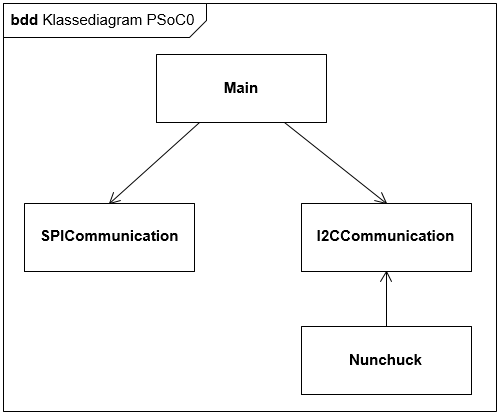
\includegraphics[width=.7\textwidth]{DesignOgImplementering/images/PSoC0KlassediagramOversigt}
	\caption{Klassediagram oversigt for PSoC0}
	\label{figure:klassediagramPSoC0}
\end{figure}

\begin{figure}[H]
	\centering
	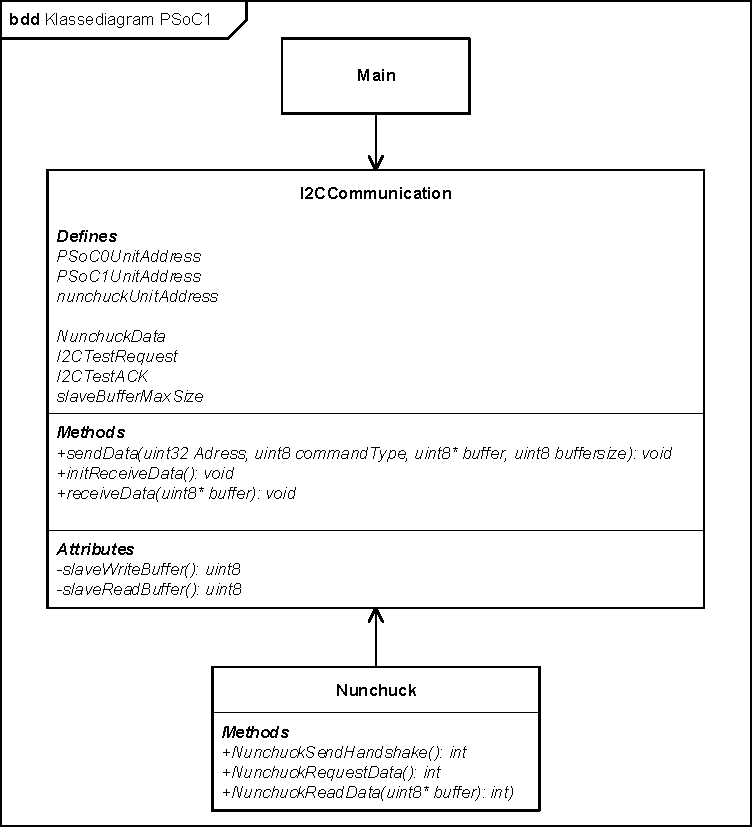
\includegraphics[width=.7\textwidth]{DesignOgImplementering/images/PSoC1KlassediagramOversigt}
	\caption{Klassediagram oversigt for PSoC1}
	\label{figure:klassediagramPSoC1}
\end{figure}

\subsection{I2CCommunication}
I dette afsnit vil softwaren der omhandler I2C-kommunikation blive beskrevet. Dette inkluderer et klassediagram, samt en klassebeskrivelse.
\subsubsection{Klassediagram}
På figur \ref{figure:klassediagramI2CCommunication} ses klassediagrammet for I2CCommunication. 
\begin{figure}[H]
	\centering
	%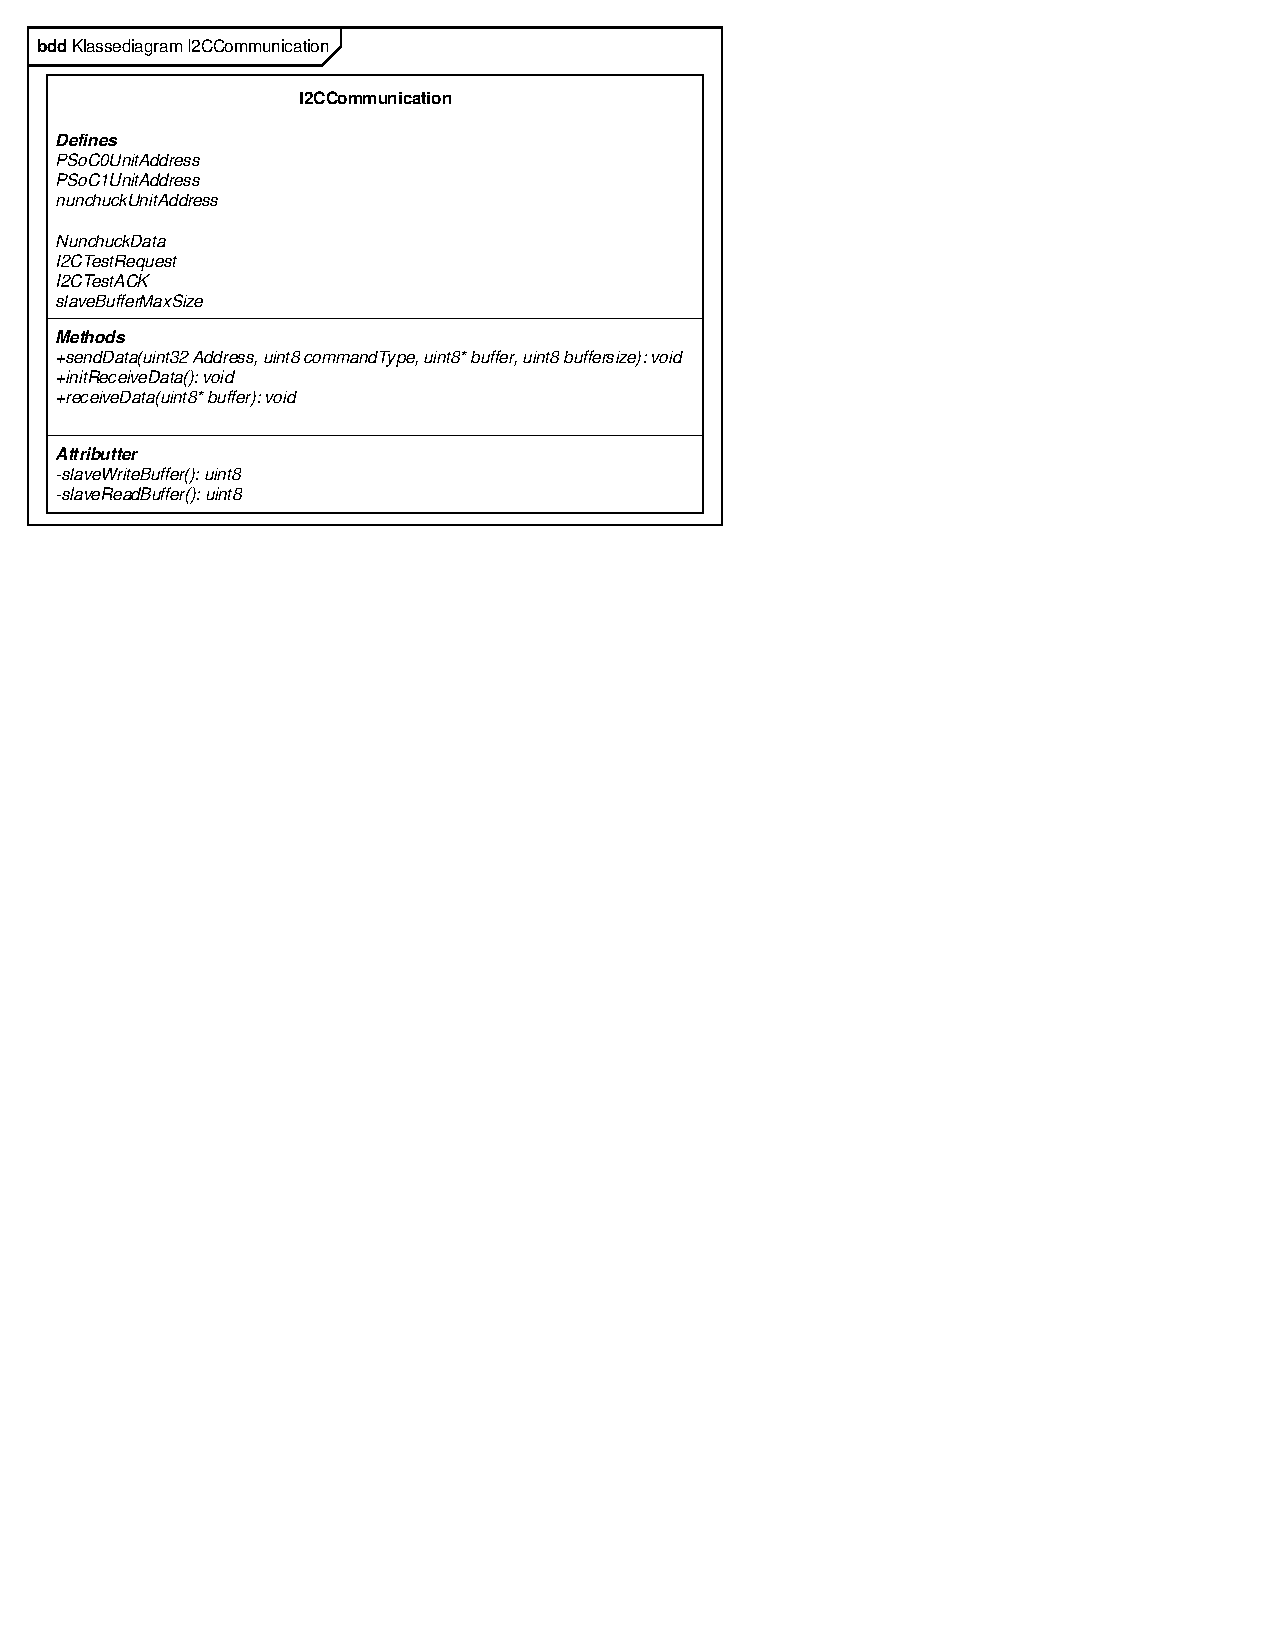
\includegraphics[width=0.9\textwidth, trim={0 19cm 9cm 0},clip]{DesignOgImplementering/images/I2CCommunication.pdf}
	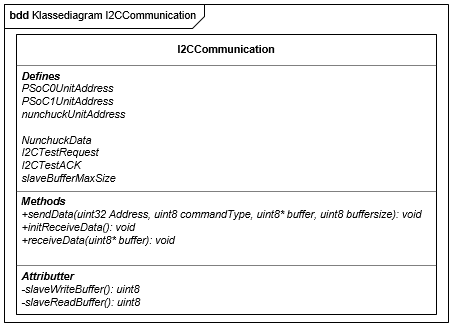
\includegraphics[]{DesignOgImplementering/images/I2CCommunication}
	%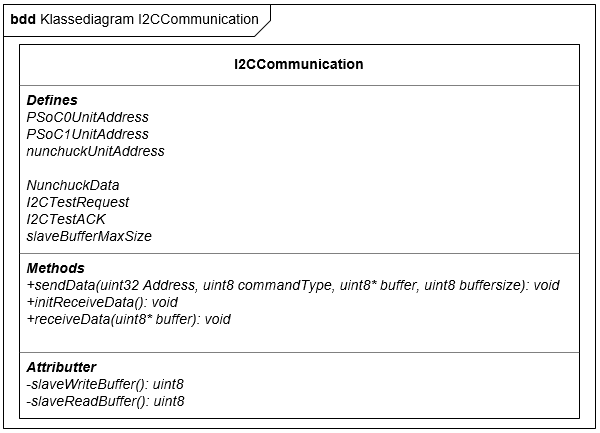
\includegraphics[width =0.9\textwidth]{DesignOgImplementering/images/I2CCommunication2}
	\caption{Klassediagram for I2CCommunication klassen}
	\label{figure:klassediagramI2CCommunication}
\end{figure}

\subsection{Nunchuck}
I dette afsnit vil softwaren der specifikt omhandler kommunikationen mellem PSoC0 og Nunchucken blive beskrevet. Dette gøres vha. et klassediagram og klassebeskrivelser.

\subsubsection{Klassediagram}
På figur \ref{figure:NunchuckKlassediagram} ses klassediagrammet for Nunchuck klassen.

\begin{figure}[H]
	\centering
	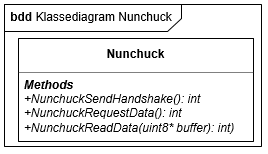
\includegraphics[]{DesignOgImplementering/images/nunchuck}
	\caption{Klassediagram for klassen Nunchuck}
	\label{figure:NunchuckKlassediagram}
\end{figure}

\subsection{SPI - PSoC}
I dette afsnit vil softwaren der specifikt omhandler SPI-kommunikationen mellem PSoC0 og DevKit8000 blive beskrevet. Dette gøres vha. et klassediagram og klassebeskrivelser

\subsubsection{Klassediagram}
På figur \ref{figure:KlassediagramSPICommunication} ses klassediagrammet over SPICommunication klassen.

\begin{figure}[H]
	\centering
	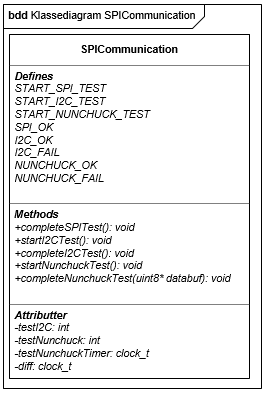
\includegraphics[]{DesignOgImplementering/images/SPICommunication}
	\caption{Klassediagram over klassen SPICommunication}
	\label{figure:KlassediagramSPICommunication}
\end{figure}


\subsection{PSoC - Affyringsmekanisme}
 
Affyringsmekanismen består udover hardware og mekanik også flere software dele, som er programmeret på PSoC2. Til rotationsdetektorens operationsforstærker er der anvendt en, der er indbygget i PSoC'en. For at se hvilke pins den er ført ud til, se dokumentationen !!!ref!!. Derudover styres bl.a. interupt og PWM signaler i forbindelse med affyringsmekanismen, ved hjælp af PSoC2.
På figur \ref{fig:aktivitetsdiagramDetektor} ses kodesekvensen som køres, når kanonen skal affyres. 
 
\begin{figure}[H]
	\centering
	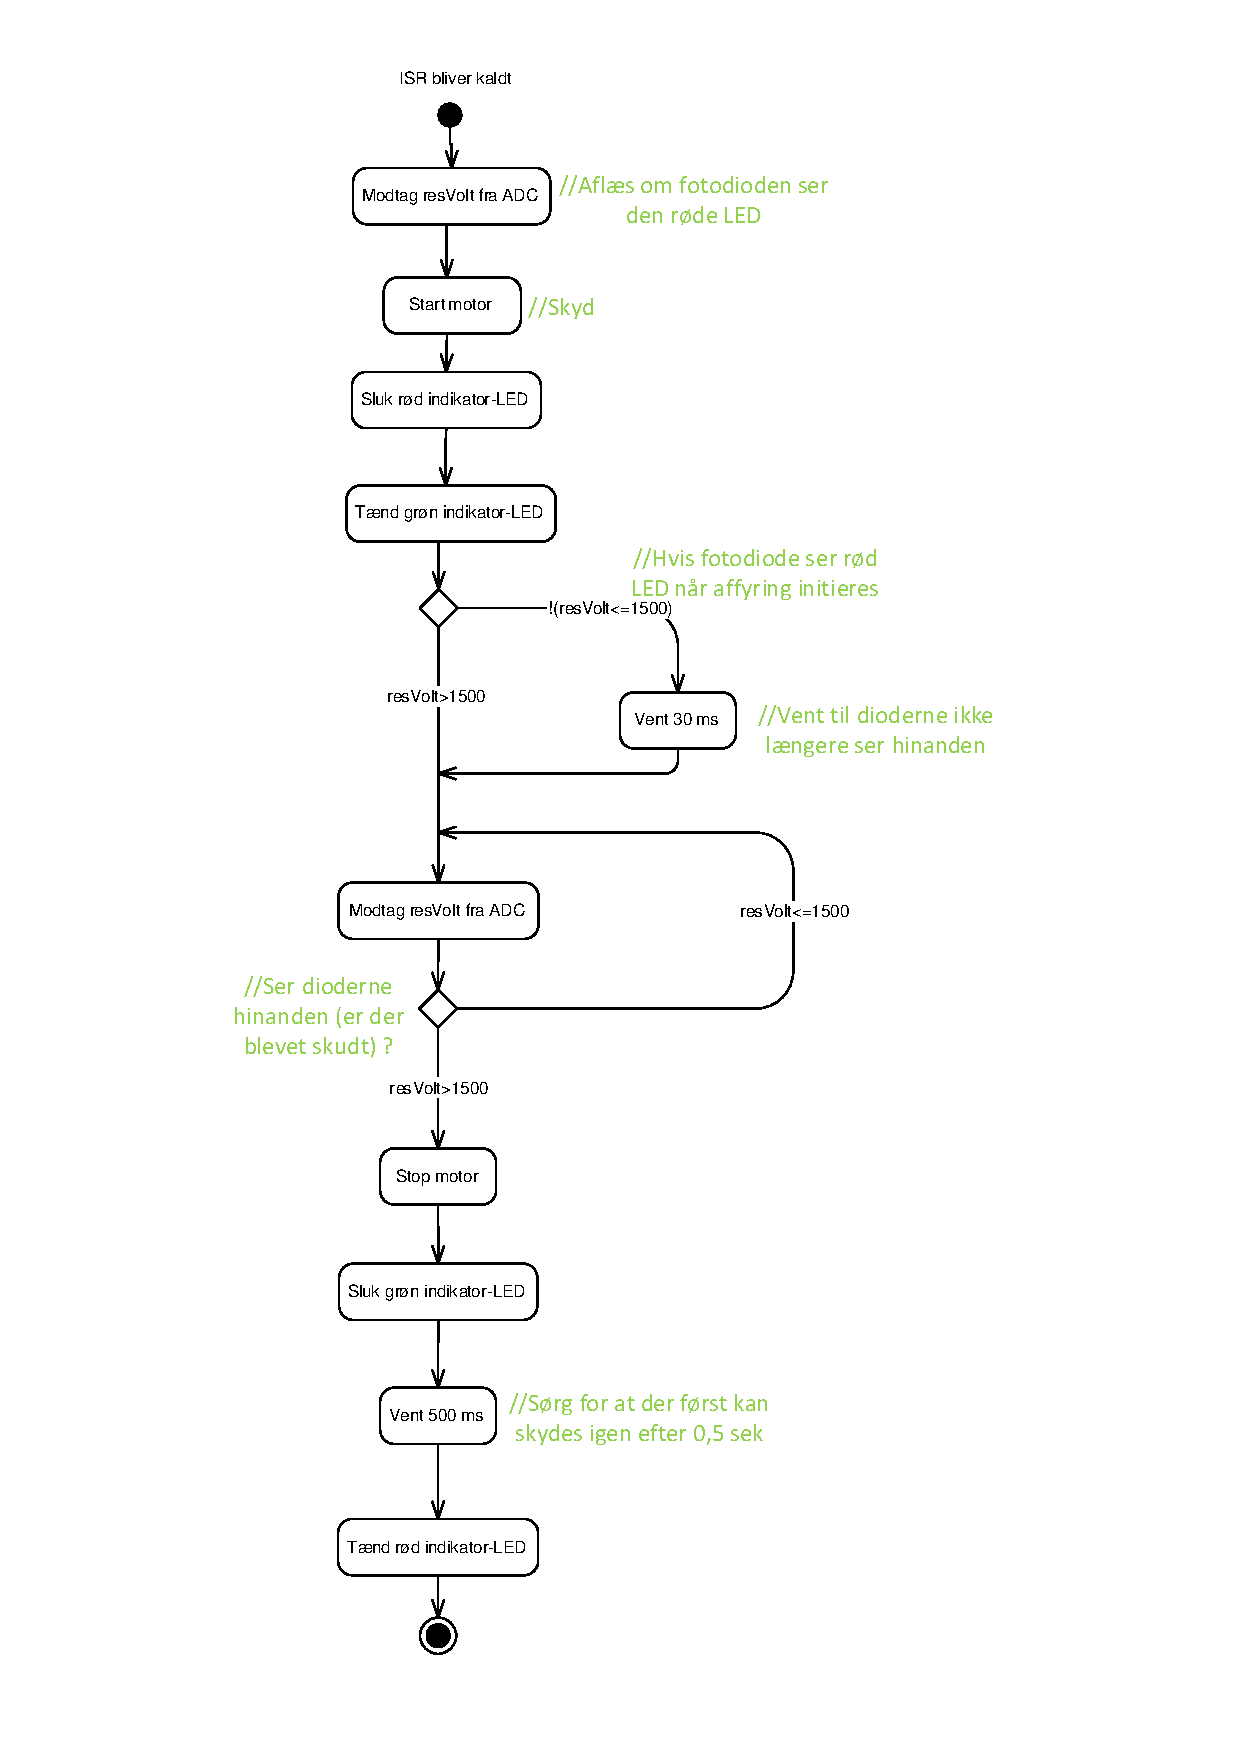
\includegraphics[width=\textwidth]{Afsnit/DesignOgImplementering/images/Aktivitetsdiagram_ISR_detektor}
	\caption{Interface driver for UC2}
	\label{fig:aktivitetsdiagramDetektor}
\end{figure}

For at affyringssekvensen kører, skal der modtages et interrupt. Det sker, når brugeren affyrer kanonen. PSoC????? sender et højt signal, som går ind på en inputpind på PSoC2, som så er programmeret til at trigge på rising edge og derved køre interruptrutinen. 
Det første der sker i interruptrutinen er, at ADC-værdien aflæses som en spænding i millivolt. Den lægges over i variablen "resVolt". Så startes motoren, derved begynder kanonen at affyre. PSoC'ens røde LED er som udgangspunkt tændt, når der ikke affyres, når interruptet kommer, slukkes den, og den grønne PSoC-LED tændes i stedet, for at indikere at interruptrutinen køres. 
Dernæst anvendes spændingen fra resVolt, der blev aflæst fra ADC'en så til at vurdere om fotodioden, kan se lyset fra den røde LED. Når de ikke kan se hinanden er spændingen 500 mV, og når de kan se hinanden er spædningen mellem 4000 og 5000 mV. Normalt indikerer det, at de kan se hinanden, at affyringen er færdig, og at motoren skal stoppes, men hvis de kan se hinanden på dette tidspunkt ved interruptets start, betyder det, at de, inden affyringen er startet, allerede er placeret så de kan se hinanden. Hvis det er tilfældet køres et delay på 30 ms, for at sikre at motoren er drejet, så de igen ikke kan se hinanden. Derefter aflæses spændingen ved ADC'en igen - nu for at tjekke om affyringen er afsluttet. Aflæsningen gentages indtil fotodioden kan se den røde LED, og motoren dermed skal stoppes. Affyringen sker på langt under et sekund, og det er derfor ikke problematisk med polling. Alternativt, hvis affyringen varede længere tid, kunne det have været implementeret med et interrupt, men i dette tilfælde kan det klares ved at tjekke ADC'en flere gange. 

Når motoren er stoppet, slukkes den grønne PSoC-LED, og der køres et delay på 500 ms, så der går et halvt sekund, inden der igen kan skydes. Derved undgås det, at kanonen affyres med det samme igen, hvis triggeren ved en fejl ikke er sluppet. Som det sidste tændes den røde PSoC LED, som indikator på, at kanonen igen er klar til at blive affyret. 

Både PWM-signalet til affyring af motoren og til generering af 10 kHz til den røde LED styres af PSoC2. De to PWM-blokke deles om en clock, der er sat til en frekvens på 2,5 MHz. PWM til den røde LED, har en periode på 250, dermed bliver PWM-signalet 10 kHz. Derudover er dutycyclen for LED'en 10 \%. PWM-signalet til motoren har en periode på 75, derved bliver frekvensen 33,33 kHz. En DC-motor skal gerne styres af et PWM-signal på over 20 kHz, for at rotere uden problemer. Dermed passer de 33,33 kHz godt. 
